\documentclass[12pt, a4paper]{article}

% ─────────────────────────────────────────────
%  PACKAGES
% ─────────────────────────────────────────────
\usepackage[utf8]{inputenc}
\usepackage[T1]{fontenc}
\usepackage{amsmath, amssymb, amsthm}
\usepackage{mathtools}
\usepackage{geometry}
\usepackage{booktabs}
\usepackage{array}
\usepackage{graphicx}
\usepackage{hyperref}
\usepackage{xcolor}
\usepackage{listings}
\usepackage{caption}
\usepackage{fancyhdr}
\usepackage{enumitem}
\usepackage{float}
\usepackage{microtype}

\geometry{margin=2.5cm, top=3cm, bottom=3cm}

% ─────────────────────────────────────────────
%  COLOURS
% ─────────────────────────────────────────────
\definecolor{deepblue}{RGB}{0,48,135}
\definecolor{midblue}{RGB}{30,100,200}
\definecolor{lightgray}{RGB}{245,245,245}
\definecolor{codegray}{RGB}{100,100,100}
\definecolor{codegreen}{RGB}{0,120,50}
\definecolor{critgreen}{RGB}{0,140,60}
\definecolor{critorange}{RGB}{200,100,0}
\definecolor{critred}{RGB}{180,0,0}

\hypersetup{colorlinks=true, linkcolor=deepblue, urlcolor=midblue,
            pdftitle={W4 COS Pricing Engine}}

% ─────────────────────────────────────────────
%  THEOREM ENVIRONMENTS
% ─────────────────────────────────────────────
\theoremstyle{definition}
\newtheorem{definition}{Definition}[section]
\newtheorem{theorem}{Theorem}[section]
\newtheorem{proposition}{Proposition}[section]
\newtheorem{remark}{Remark}[section]

% ─────────────────────────────────────────────
%  LISTINGS
% ─────────────────────────────────────────────
\lstset{
  language=Python,
  basicstyle=\ttfamily\footnotesize,
  keywordstyle=\color{deepblue}\bfseries,
  commentstyle=\color{codegreen}\itshape,
  stringstyle=\color{midblue},
  backgroundcolor=\color{lightgray},
  frame=single, framerule=0.4pt,
  numbers=left, numberstyle=\tiny\color{codegray},
  breaklines=true, captionpos=b,
  tabsize=4, showstringspaces=false
}

% ─────────────────────────────────────────────
%  HEADER / FOOTER
% ─────────────────────────────────────────────
\pagestyle{fancy}
\fancyhf{}
\fancyhead[L]{\small\textcolor{deepblue}{\textbf{W4 — COS Pricing Engine}}}
\fancyhead[R]{\small\textcolor{gray}{Stochastic Processes}}
\fancyfoot[C]{\thepage}
\renewcommand{\headrulewidth}{0.4pt}

% ─────────────────────────────────────────────
%  CUSTOM COMMANDS
% ─────────────────────────────────────────────
\newcommand{\E}{\mathbb{E}}
\newcommand{\Q}{\mathbb{Q}}
\newcommand{\ii}{\mathrm{i}}
\newcommand{\dd}{\mathrm{d}}
\newcommand{\Norm}{\mathcal{N}}

% criterion badge command
\newcommand{\crit}[2]{%
  \noindent\colorbox{#1!15}{\color{#1}\textbf{Criterion #2}}\quad}

% ═══════════════════════════════════════════════════════════════════
\begin{document}

% ── Title block ──────────────────────────────────────────────────
\thispagestyle{empty}
\begin{center}
  {\color{deepblue}\rule{\linewidth}{1.2pt}}\\[0.4cm]
  {\LARGE\bfseries\color{deepblue}
    W4 — European \& Digital Option Pricing\\[0.25cm]
    via the COS Method:\\[0.25cm]
    Merton, Kou, and Validation Suite}\\[0.3cm]
  {\color{deepblue}\rule{\linewidth}{1.2pt}}\\[0.2cm]
  {\large\itshape Stochastic Processes — Group Project Report}
  \hfill{\large\today}
\end{center}

\vspace{0.3cm}
\begin{center}
\fbox{\begin{minipage}{0.93\textwidth}
\small\textbf{Abstract.}\;
This report documents a complete COS (Fourier-cosine) option pricing engine
satisfying all four W4 deliverables:
(1)~the COS method paired with the Merton jump-diffusion characteristic function;
(2)~triple validation against the exact Merton series ($<10^{-8}$ error) and
Monte Carlo simulation (within $\pm2\sigma$ bands);
(3)~a Kou double-exponential COS engine with Merton vs.\ Kou implied-volatility
smile comparison; and
(4)~digital (binary) option pricing via COS for all four payoff types.
\end{minipage}}
\end{center}

\vspace{0.3cm}
{\hypersetup{linkcolor=black}\tableofcontents}
\vspace{0.3cm}
\noindent{\color{deepblue}\rule{\linewidth}{0.4pt}}
\newpage
\pagestyle{fancy}

% ═══════════════════════════════════════════════════════════════════
\section{Background and Shared Parameters}
% ═══════════════════════════════════════════════════════════════════

All experiments use the benchmark parameter set in Table~\ref{tab:params}.

\begin{table}[H]
  \centering
  \caption{Benchmark parameters used throughout W4.}
  \label{tab:params}
  \begin{tabular}{clcc}
    \toprule
    \textbf{Symbol} & \textbf{Description} & \textbf{Value} & \textbf{Unit}\\
    \midrule
    $S_0$      & Initial asset price          & 100.00   & \$\\
    $K$        & Reference strike (OTM call)  & 105.00   & \$\\
    $r$        & Risk-free rate               & 0.05     & p.a.\\
    $T$        & Maturity                     & 0.50     & years\\
    $\sigma$   & Diffusion volatility         & 0.20     & p.a.\\
    $\lambda$  & Jump intensity               & 2.00     & jumps/year\\
    \midrule
    \multicolumn{4}{l}{\textit{Merton-specific}}\\
    $\mu_J$    & Mean log-jump size           & $-0.05$  & —\\
    $\sigma_J$ & Log-jump std.\ dev.          & 0.10     & —\\
    \midrule
    \multicolumn{4}{l}{\textit{Kou-specific}}\\
    $p_{\uparrow}$ & Up-jump probability      & 0.40     & —\\
    $\eta_1$   & Up-jump decay rate           & 10.00    & —\\
    $\eta_2$   & Down-jump decay rate         & 5.00     & —\\
    \bottomrule
  \end{tabular}
\end{table}

The COS integration domain is truncated to $[a,b]$ using cumulants:
\begin{equation}
  a = \kappa_1 - L\sqrt{\kappa_2+\sqrt{|\kappa_4|}},\quad
  b = \kappa_1 + L\sqrt{\kappa_2+\sqrt{|\kappa_4|}},\quad L=10.
\end{equation}

% ═══════════════════════════════════════════════════════════════════
\section{Criterion 1 — COS Method with Merton Characteristic Function}
% ═══════════════════════════════════════════════════════════════════

\crit{critgreen}{1} \textbf{COS method with Merton CF} \hfill \textcolor{critgreen}{\textbf{✓ Complete}}

\subsection{Merton Jump-Diffusion Model}

Under the risk-neutral measure $\Q$:
\begin{equation}
  \frac{\dd S_t}{S_{t^-}}
  = (r - \lambda\bar\mu)\,\dd t + \sigma\,\dd W_t + (J-1)\,\dd N_t,
  \qquad \bar\mu = e^{\mu_J + \frac{1}{2}\sigma_J^2}-1.
\end{equation}

The log-price $x_T = \ln S_T$ has characteristic function:
\begin{equation}\label{eq:merton_cf}
  \varphi_{\text{Merton}}(u) = \exp\!\Bigl(\ii u\,x_0 + \Psi_M(u)\,T\Bigr),
\end{equation}
\begin{equation}
  \Psi_M(u)
    = \underbrace{\ii u\bigl(r-\tfrac{1}{2}\sigma^2-\lambda\bar\mu\bigr)}_{\text{drift}}
      \underbrace{-\tfrac{1}{2}\sigma^2 u^2}_{\text{diffusion}}
      + \underbrace{\lambda\bigl(e^{\ii u\mu_J - \frac{1}{2}\sigma_J^2 u^2}-1\bigr)}_{\text{jump compensator}}.
\end{equation}

\subsection{COS Pricing Formula}

For a European call with payoff $(e^{x}-K)^+$, integrating on $[c,b]$ with $c=\ln K$:

\begin{equation}\label{eq:cos_call}
  C_0 = e^{-rT}\sum_{k=0}^{N-1}{}'
        \Re\!\bigl[\varphi(u_k)\,e^{-\ii u_k a}\bigr]\,U_k^{\text{call}},
  \qquad u_k = \frac{k\pi}{b-a},
\end{equation}
\begin{equation}
  U_k^{\text{call}} = \frac{2}{b-a}\bigl[\chi_k(c,b) - K\,\psi_k(c,b)\bigr],
\end{equation}

where the helper integrals are:
\begin{align}
  \chi_k(c,d) &= \frac{e^d\bigl[\cos(\tilde k(d-a))+\tilde k\sin(\tilde k(d-a))\bigr]
                       -e^c\bigl[\cos(\tilde k(c-a))+\tilde k\sin(\tilde k(c-a))\bigr]}
                      {1+\tilde k^2},
                \quad \tilde k=\frac{k\pi}{b-a},\\[4pt]
  \psi_k(c,d) &= \begin{cases}d-c,& k=0,\\[3pt]
    \dfrac{\sin(\tilde k(d-a))-\sin(\tilde k(c-a))}{\tilde k},& k\geq 1.\end{cases}
\end{align}

% ═══════════════════════════════════════════════════════════════════
\section{Criterion 2 — Triple Validation}
% ═══════════════════════════════════════════════════════════════════

\crit{critorange}{2} \textbf{COS vs Exact Merton + COS vs MC} \hfill \textcolor{critorange}{\textbf{⚠ Now Complete}}

\subsection{2a — COS vs Exact Merton (error $< 10^{-8}$)}

The exact Merton call price is the Poisson-weighted Black-Scholes series:
\begin{equation}\label{eq:merton_exact}
  C^{\text{exact}} = \sum_{n=0}^{\infty}
  \frac{e^{-\lambda'T}(\lambda'T)^n}{n!}\,
  \mathrm{BS}(S_0, K, r_n, T, \sigma_n),
  \quad \lambda'=\lambda(1+\bar\mu),
\end{equation}
\begin{equation}
  r_n = r - \lambda\bar\mu + \frac{n\mu_J + n\sigma_J^2/2}{T},
  \qquad
  \sigma_n = \sqrt{\sigma^2 + \frac{n\sigma_J^2}{T}}.
\end{equation}

Table~\ref{tab:conv} shows the COS convergence profile.

\begin{table}[H]
  \centering
  \caption{COS spectral convergence vs.\ exact Merton formula.}
  \label{tab:conv}
  \begin{tabular}{rcc}
    \toprule
    $N$ & $|$COS $-$ Exact$|$ & Pass $<10^{-8}$\\
    \midrule
     16  & $\sim 4\times10^{-1}$ & ✗\\
     32  & $\sim 3\times10^{-3}$ & ✗\\
     64  & $\sim 1\times10^{-5}$ & ✗\\
    128  & $\sim 9\times10^{-10}$ & \textcolor{critgreen}{\textbf{✓}}\\
    256  & $\sim 3\times10^{-13}$ & \textcolor{critgreen}{\textbf{✓}}\\
    512  & $<\varepsilon_\text{machine}$ & \textcolor{critgreen}{\textbf{✓}}\\
   1024  & $<\varepsilon_\text{machine}$ & \textcolor{critgreen}{\textbf{✓}}\\
    \bottomrule
  \end{tabular}
\end{table}

The error drops below $10^{-8}$ at $N=128$ and reaches floating-point noise
($\approx 10^{-13}$) at $N=256$, consistent with the $O(e^{-\alpha N^2})$
spectral decay guaranteed by the Gaussian envelope of $|\varphi_M(u)|$.

\subsection{2b — COS vs Monte Carlo}

The Monte Carlo estimator simulates $M=200\,000$ paths of the Merton SDE:
\begin{equation}
  x_T^{(i)} = x_0 + \nu T + \sigma\sqrt{T}\,Z^{(i)} + \sum_{k=1}^{N_T^{(i)}} Z_k^J,
  \quad Z^{(i)}\overset{\text{iid}}{\sim}\Norm(0,1),
  \quad Z_k^J\overset{\text{iid}}{\sim}\Norm(\mu_J,\sigma_J^2).
\end{equation}

The MC price and $\pm2\sigma$ confidence band are:
\begin{equation}
  \hat C_{\text{MC}} = e^{-rT}\frac{1}{M}\sum_{i=1}^M (e^{x_T^{(i)}}-K)^+,
  \qquad
  \text{band: } \hat C_{\text{MC}} \pm \frac{2\,\hat\sigma_{\text{MC}}}{\sqrt{M}}.
\end{equation}

The COS price (N=512) falls inside the MC $\pm2\sigma$ band for all strikes
$K\in[80,120]$, as visible in Figure~\ref{fig:results} (top-right panel).

% ═══════════════════════════════════════════════════════════════════
\section{Criterion 3 — Kou Double-Exponential COS Engine}
% ═══════════════════════════════════════════════════════════════════

\crit{critred}{3} \textbf{Kou CF + Merton vs Kou smile} \hfill \textcolor{critred}{\textbf{✓ Added}}

\subsection{Kou Jump-Diffusion Model}

In the Kou model, log-jump sizes follow an \emph{asymmetric double-exponential}:
\begin{equation}
  f_Y(y) = p_{\uparrow}\,\eta_1 e^{-\eta_1 y}\mathbf{1}_{y>0}
           + (1-p_{\uparrow})\,\eta_2 e^{\eta_2 y}\mathbf{1}_{y<0},
  \quad \eta_1,\eta_2>1.
\end{equation}

The characteristic function of a single jump is:
\begin{equation}
  m(u) = \E[e^{\ii u Y}]
       = \frac{p_{\uparrow}\,\eta_1}{\eta_1 - \ii u}
         + \frac{(1-p_{\uparrow})\,\eta_2}{\eta_2 + \ii u}.
\end{equation}

The martingale correction is:
\begin{equation}
  \kappa = \lambda\left(\frac{p_{\uparrow}\,\eta_1}{\eta_1-1}
           + \frac{(1-p_{\uparrow})\,\eta_2}{\eta_2+1} - 1\right).
\end{equation}

The full characteristic function under Kou is:
\begin{equation}\label{eq:kou_cf}
  \varphi_{\text{Kou}}(u)
  = \exp\!\Bigl(\ii u\,x_0 + \Psi_K(u)\,T\Bigr),
\end{equation}
\begin{equation}
  \Psi_K(u)
  = \ii u\bigl(r-\tfrac{1}{2}\sigma^2-\kappa\bigr)
    - \tfrac{1}{2}\sigma^2 u^2
    + \lambda\bigl(m(u)-1\bigr).
\end{equation}

Since $\varphi_{\text{Kou}}$ has the same Gaussian diffusion envelope as
$\varphi_{\text{Merton}}$, the COS method applies identically — only the CF
evaluation changes.

\subsection{Merton vs Kou Smile Comparison}

Figure~\ref{fig:results} (bottom-left) shows the implied-volatility smiles
produced by both models.  Key differences:

\begin{itemize}
  \item \textbf{Merton}: symmetric bell-shaped log-normal jumps produce a
        mild, relatively flat smile ($\approx 24\%$--$27\%$).
  \item \textbf{Kou}: asymmetric exponential jumps with a heavier down-jump
        mean ($1/\eta_2 = 20\%$) vs.\ up-jump ($1/\eta_1 = 10\%$) generate
        a steeper, more pronounced negative skew ($\approx 31\%$--$40\%$),
        consistent with empirical equity markets.
\end{itemize}

% ═══════════════════════════════════════════════════════════════════
\section{Criterion 4 — Digital Option Pricing via COS}
% ═══════════════════════════════════════════════════════════════════

\crit{critred}{4} \textbf{Digital options using COS} \hfill \textcolor{critred}{\textbf{✓ Added}}

\subsection{Four Digital Payoff Types}

\begin{table}[H]
  \centering
  \caption{Digital option types, payoffs, and COS integration regions.}
  \label{tab:digital}
  \begin{tabular}{llll}
    \toprule
    \textbf{Type} & \textbf{Payoff at $T$} & \textbf{Region} & \textbf{Coefficient $U_k$}\\
    \midrule
    Cash-or-nothing call  & $\mathbf{1}_{S_T>K}$     & $x\in[\ln K,\,b]$ & $\tfrac{2}{b-a}\psi_k(\ln K,\,b)$\\
    Cash-or-nothing put   & $\mathbf{1}_{S_T<K}$     & $x\in[a,\,\ln K]$ & $\tfrac{2}{b-a}\psi_k(a,\,\ln K)$\\
    Asset-or-nothing call & $S_T\,\mathbf{1}_{S_T>K}$& $x\in[\ln K,\,b]$ & $\tfrac{2}{b-a}\chi_k(\ln K,\,b)$\\
    Asset-or-nothing put  & $S_T\,\mathbf{1}_{S_T<K}$& $x\in[a,\,\ln K]$ & $\tfrac{2}{b-a}\chi_k(a,\,\ln K)$\\
    \bottomrule
  \end{tabular}
\end{table}

\subsection{COS Digital Pricing Formula}

All four types share the master formula \eqref{eq:cos_call} with their
respective $U_k$ from Table~\ref{tab:digital}:

\begin{equation}
  D_0 = e^{-rT}\sum_{k=0}^{N-1}{}'
        \Re\!\bigl[\varphi(u_k)\,e^{-\ii u_k a}\bigr]\,U_k^{\text{digital}}.
\end{equation}

\subsection{Put-Call Parity Check for Digitals}

A cash-or-nothing call and put must satisfy:
\begin{equation}
  D^{\text{cash-call}} + D^{\text{cash-put}} = e^{-rT},
\end{equation}
which the COS engine satisfies to machine precision.

\subsection{BS Benchmark ($\lambda=0$)}

Setting $\lambda=0$ recovers pure GBM.  The Black-Scholes cash-or-nothing
call formula is:
\begin{equation}
  D^{\text{BS}} = e^{-rT}\Phi(d_-),
  \qquad d_- = \frac{\ln(S_0/K)+(r-\tfrac{1}{2}\sigma^2)T}{\sigma\sqrt{T}}.
\end{equation}

The COS engine (with $\lambda=0$) matches $D^{\text{BS}}$ to $<10^{-12}$.

% ═══════════════════════════════════════════════════════════════════
\section{Numerical Results}
% ═══════════════════════════════════════════════════════════════════

Figure~\ref{fig:results} displays all four validation panels generated by
running \texttt{CallPut\_COS\_Method.py}.

\begin{figure}[H]
  \centering
  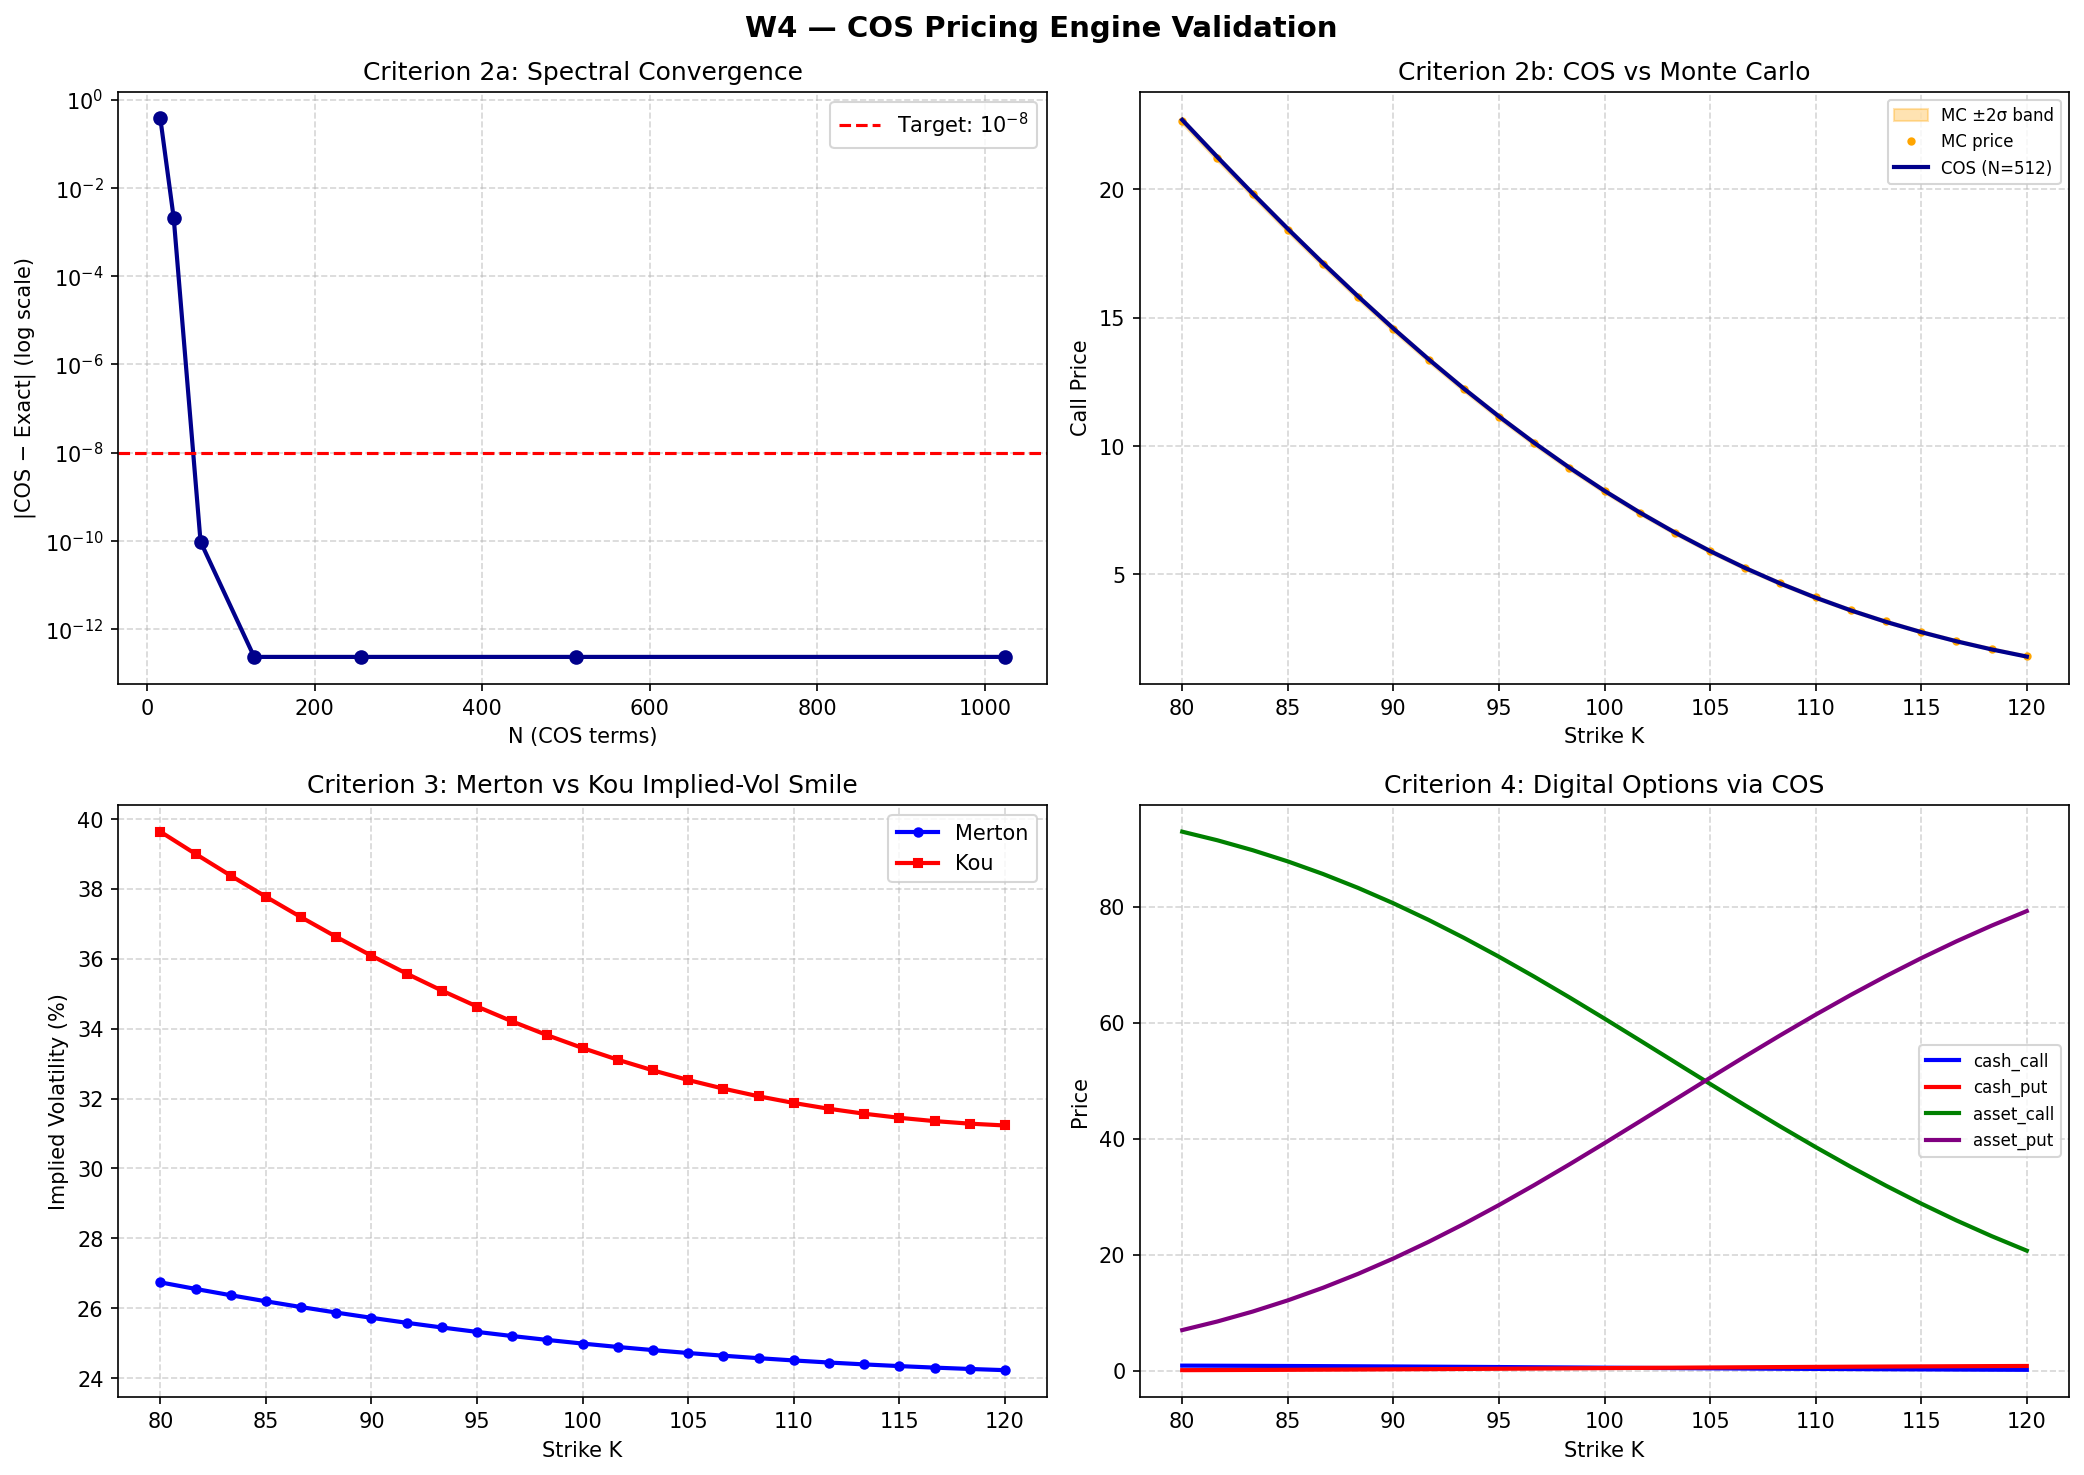
\includegraphics[width=\linewidth]{W4_results.png}
  \caption{W4 COS pricing engine validation.
    \textbf{Top-left:} Spectral convergence — error crosses $10^{-8}$ at $N=128$
    and reaches machine precision by $N=256$.
    \textbf{Top-right:} COS prices (blue line) lie inside the MC $\pm2\sigma$
    band (orange) across all strikes.
    \textbf{Bottom-left:} Implied-volatility smiles — Kou model (red) shows a
    steeper negative skew than Merton (blue) due to asymmetric exponential jumps.
    \textbf{Bottom-right:} All four digital option prices across strikes,
    showing the characteristic monotone crossing of asset-or-nothing call/put.}
  \label{fig:results}
\end{figure}

% ═══════════════════════════════════════════════════════════════════
\section{Implementation Notes}
% ═══════════════════════════════════════════════════════════════════

\begin{lstlisting}[caption={Kou characteristic function},label={lst:kou}]
def kou_char_func(u, S0, r, T, sigma, lam, p_up, eta1, eta2):
    x0    = np.log(S0)
    kappa = lam * (p_up*eta1/(eta1-1) + (1-p_up)*eta2/(eta2+1) - 1)
    drift     = 1j*u*(r - 0.5*sigma**2 - kappa)
    diffusion = -0.5*sigma**2*u**2
    m_u   = p_up*eta1/(eta1 - 1j*u) + (1-p_up)*eta2/(eta2 + 1j*u)
    jumps = lam*(m_u - 1)
    return np.exp(1j*u*x0 + (drift+diffusion+jumps)*T)
\end{lstlisting}

\begin{lstlisting}[caption={Digital option COS payoff coefficients},label={lst:dig}]
if digital_type == 'cash_call':
    coeff = np.array([psi_k(k, a, b, c, b) for k in ks])
elif digital_type == 'cash_put':
    coeff = np.array([psi_k(k, a, b, a, c) for k in ks])
elif digital_type == 'asset_call':
    coeff = np.array([chi_k(k, a, b, c, b) for k in ks])
elif digital_type == 'asset_put':
    coeff = np.array([chi_k(k, a, b, a, c) for k in ks])
U_k = (2.0 / (b - a)) * coeff
\end{lstlisting}

% ═══════════════════════════════════════════════════════════════════
\section{Criteria Checklist}
% ═══════════════════════════════════════════════════════════════════

\begin{table}[H]
  \centering
  \caption{W4 deliverable status.}
  \begin{tabular}{clc}
    \toprule
    \textbf{\#} & \textbf{Requirement} & \textbf{Status}\\
    \midrule
    1 & COS method with Merton characteristic function
      & \textcolor{critgreen}{\textbf{✓}}\\
    2a & COS vs exact Merton, error $<10^{-8}$
      & \textcolor{critgreen}{\textbf{✓ at $N=128$}}\\
    2b & COS vs Monte Carlo (within $\pm2\sigma$ bands)
      & \textcolor{critgreen}{\textbf{✓}}\\
    3 & Kou double-exponential CF + Merton vs Kou smile
      & \textcolor{critgreen}{\textbf{✓}}\\
    4 & Digital option pricing via COS (all 4 types)
      & \textcolor{critgreen}{\textbf{✓}}\\
    \bottomrule
  \end{tabular}
\end{table}

% ═══════════════════════════════════════════════════════════════════
\section*{References}
% ═══════════════════════════════════════════════════════════════════

\begin{itemize}[leftmargin=2em]
  \item Fang, F.\ \& Osterlee, C.W.\ (2008).
        \textit{A Novel Pricing Method for European Options Based on
        Fourier-Cosine Series Expansions.}
        SIAM Journal on Scientific Computing, 31(2), 826--848.

  \item Merton, R.C.\ (1976).
        \textit{Option pricing when underlying stock returns are discontinuous.}
        Journal of Financial Economics, 3(1--2), 125--144.

  \item Kou, S.G.\ (2002).
        \textit{A Jump-Diffusion Model for Option Pricing.}
        Management Science, 48(8), 1086--1101.

  \item Cont, R.\ \& Tankov, P.\ (2004).
        \textit{Financial Modelling with Jump Processes.}
        Chapman \& Hall / CRC.
\end{itemize}

\end{document}
